\subsection{Analog-to-Digital Converter}
Mikrokontrolleren indeholder en SAR ADC, som gør det muligt at konvertere det analoge signal til et digitalt. Der ønskes en konfigurering af 3 analoge kanaler, herunder Y-aksen på begge accelerometre samt EMG-forstærkeren. Opsætningen af ADC'en på mikrokontrolleren fremgår af \autoref{fig:ADC_teori}. Det ønskes at kunne læse signalerne hver for sig ved at måle single ended, hvorfor hvert input er tilkoblet $V_{ss}$. Da der ligeledes ønskes at anvende en 12 bit ADC på baggrund af kravet i \autoref{sec:ADC_teori}, indstilles denne til 12 bit. Da der anvendes single ended, svarer dette til at ADC'en anvender 11 bit, hvorfor den inddeles i $2^{11}$ svarende til 2048 niveauer. ADC'en har et arbejdsområde fra $0-5~V$. LSB'en for ADC'en kan beregnes ud fra \autoref{equ:LSB}, hvilket giver $2,44~mV$, hvis denne overskrides vil signalet gå i mætning \citep{ADC2014}. 


\begin{figure}[H]
\centering
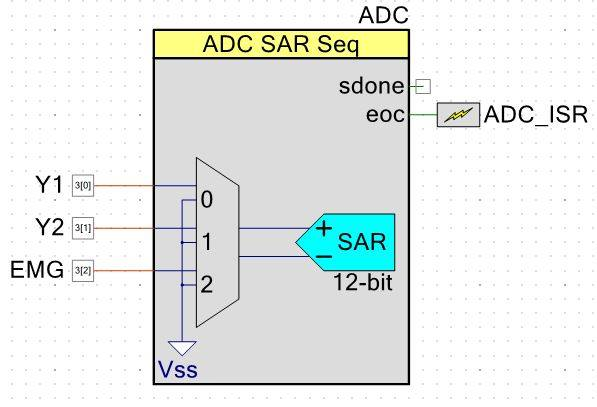
\includegraphics[width=0.5\textwidth]{figures/implementering/ADC_imp.jpg}
\caption{ADC'ens opsætning på mikrokontrolleren}
\label{fig:ADC_teori}
\end{figure}

I ADC'en er der indbygget en clock frekvens. Det er muligt at reducere konverteringstiden ved at øge ADC'ens clock frekvens. Når ADC'en skal starte på konverteringen, er det samplingstiden, der også måles som tiden i clock cycles. Der er forskellige parametre, der kan indstilles i PSoC, herunder opløsning, samplingsraten og clock frekvensen. Disse parametre bestemmer ADC'ens konverteringsrate. Konvertingstiden er den inverste af konverteringsraten. Clock frekvensen kan indstilles mellem $1000~MHz$ og $9000~MHz$.\citep{cypresspsoc42014} Da der ønskes at samples med 10 gange frekvensområdet for signalet, hvilket i følge  \autoref{sec:pilotforsoeg} er mellem 0,4 og $10~Hz$, vælges der at samples med $100~Hz$. Clockfrekvensen vælges til at have en hastighed på $1600~kHz$. Outputtet fra ADC'en er tilkoblet via eoc til ADC'ens Interrupt Service Routine (ISR), hvilket fremgår af \autoref{fig:ADC_teori}. Hvis der er sker et interrupt vil dette resultere i at de aktiverede kanaler er klar til at blive aflæst fra registrene, hvorved systemet igangsættes. \autoref{ADC2014} 


